% This file was created by matplotlib2tikz v0.5.4.
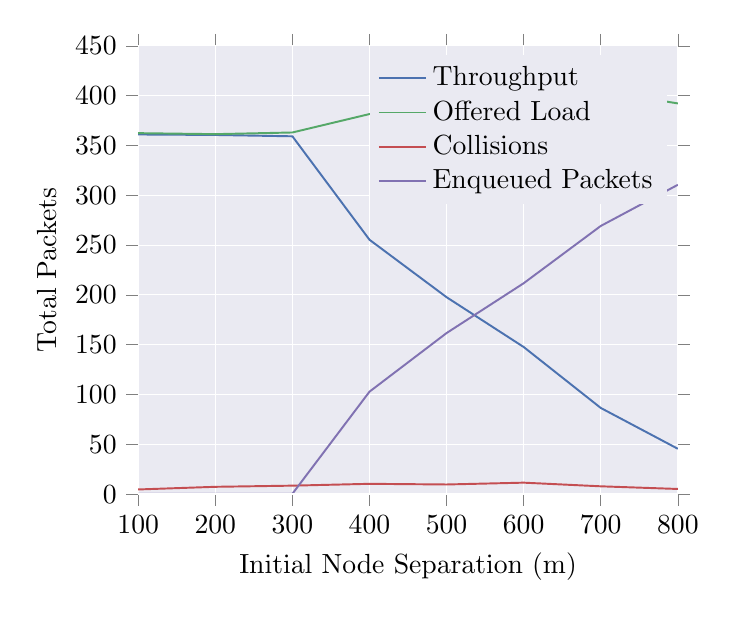
\begin{tikzpicture}

\definecolor{color1}{rgb}{0.298039215686275,0.447058823529412,0.690196078431373}
\definecolor{color0}{rgb}{0.917647058823529,0.917647058823529,0.949019607843137}
\definecolor{color3}{rgb}{0.768627450980392,0.305882352941176,0.32156862745098}
\definecolor{color2}{rgb}{0.333333333333333,0.658823529411765,0.407843137254902}
\definecolor{color4}{rgb}{0.505882352941176,0.447058823529412,0.698039215686274}

\begin{axis}[
xlabel={Initial Node Separation (m)},
ylabel={Total Packets},
xmin=100, xmax=800,
ymin=0, ymax=450,
xtick={100,200,300,400,500,600,700,800},
xticklabels={$100$,$200$,$300$,$400$,$500$,$600$,$700$,$800$},
ytick={0,50,100,150,200,250,300,350,400,450},
yticklabels={$0$,$50$,$100$,$150$,$200$,$250$,$300$,$350$,$400$,$450$},
tick align=outside,
xmajorgrids,
x grid style={white},
ymajorgrids,
y grid style={white},
axis line style={white},
axis background/.style={fill=color0},
legend style={draw=none, fill=color0},
legend cell align={left},
legend entries={{Throughput},{Offered Load},{Collisions},{Enqueued Packets}}
]
\addplot [line width=0.7000000000000001pt, color1]
table {%
100 361
200 360.5
300 359.166666666667
400 255.333333333333
500 197.666666666667
600 147.666666666667
700 86.5
800 45.5
};
\addplot [line width=0.7000000000000001pt, color2]
table {%
100 362.333333333333
200 361.333333333333
300 363
400 381.5
500 393.666666666667
600 413.166666666667
700 404.666666666667
800 392.166666666667
};
\addplot [line width=0.7000000000000001pt, color3]
table {%
100 4.66666666666667
200 7.33333333333333
300 8.5
400 10.3333333333333
500 9.66666666666667
600 11.5
700 7.83333333333333
800 5.16666666666667
};
\addplot [line width=0.7000000000000001pt, color4]
table {%
100 0.333333333333333
200 0.166666666666667
300 0.333333333333333
400 102.833333333333
500 161.666666666667
600 211.666666666667
700 269.166666666667
800 310.5
};
\path [draw=white, fill opacity=0] (axis cs:100,1)
--(axis cs:800,1);

\path [draw=white, fill opacity=0] (axis cs:1,0)
--(axis cs:1,450);

\path [draw=white, fill opacity=0] (axis cs:100,0)
--(axis cs:800,0);

\path [draw=white, fill opacity=0] (axis cs:0,0)
--(axis cs:0,450);

\end{axis}

\end{tikzpicture}